%%%%%%%%%%%%%%%%%%%%%%%%%%%%%%%%%%%%%%%%%%%%%%%%%%%%%%%%%%%%%%%%%%%%%%%%%%%%%%%%%%%%%%%%%%%%%%%%%%%%%%%%%%%%%%%%%%%%%%
\chapter{Results for separable $p$} \label{seri}%%%%%%%%%%%%%%%%%%%%%%%%%%%%%%%%%%%%%%%%%%%%%%%%%%%%%%%%%%%%%%%%%%%%%%
%%%%%%%%%%%%%%%%%%%%%%%%%%%%%%%%%%%%%%%%%%%%%%%%%%%%%%%%%%%%%%%%%%%%%%%%%%%%%%%%%%%%%%%%%%%%%%%%%%%%%%%%%%%%%%%%%%%%%%
In this whole section it is assume that $p$ is separable, and that only one processing unit is used to obtain the results. 
Section \ref{sec:sconv} will show correctness of the methods with a convergence plot. Section \ref{sec:rrest} will see if there is any correlation between $n$ and $\rho$.
Computation times for the different methods will be compared to each other and their predicted computational complexity in section \ref{sec:stimem} and \ref{sec:stimek}.
How $\gamma$ and $\epsilon$ scales with $\delta$ will be examined in section \ref{sec:div}.
%%%%%%%%%%%%%%%%%%%%%%%%%%%%%%%%%%%%%%%%%%%%%%%%%%%%%%%%%%%%%%%%%%%%%%%%%%%%%%%%%%%%%%%%%%%%%%%%%%%%%%%%%%%%%%%%%%%%%%
\section{Convergence} \label{sec:sconv}
%%%%%%%%%%%%%%%%%%%%%%%%%%%%%%%%%%%%%%%%%%%%%%%%%%%%%%%%%%%%%%%%%%%%%%%%%%%%%%%%%%%%%%%%%%%%%%%%%%%%%%%%%%%%%%%%%%%%%%
\begin{figure}[H]
        \centering
        \begin{subfigure}[b]{0.45\textwidth}
                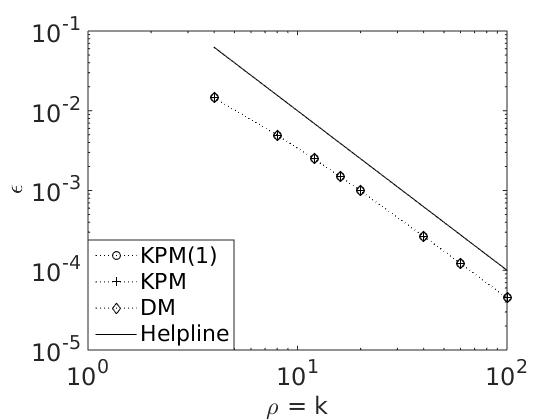
\includegraphics[width=\textwidth]{fig/s1conv1}
                \caption{function \texttt{P1}}
                \label{fig:conv1}
        \end{subfigure}%
~
        \begin{subfigure}[b]{0.45\textwidth}
                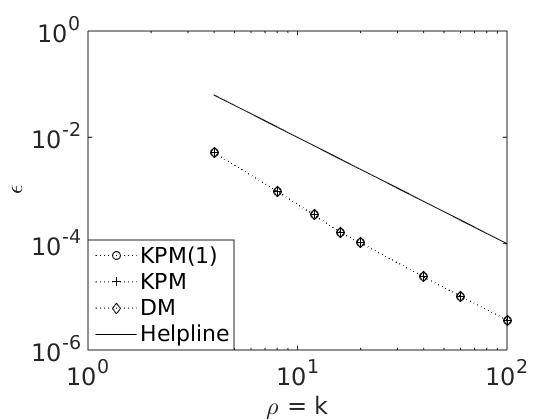
\includegraphics[width=\textwidth]{fig/s2conv2}
                \caption{function \texttt{P2}}
                \label{fig:conv2}
        \end{subfigure}
        \caption{A convergence plot for several methods with $\rho = k$. The helpline shows quadratic convergence.}\label{fig:conv}
\end{figure}
As can be seen from figure \ref{fig:conv}, all method converges quadratically and overlap perfectly, this shows that all method preforms as expected regarding convergence.
%%%%%%%%%%%%%%%%%%%%%%%%%%%%%%%%%%%%%%%%%%%%%%%%%%%%%%%%%%%%%%%%%%%%%%%%%%%%%%%%%%%%%%%%%%%%%%%%%%%%%%%%%%%%%%%%%%%%%%
\section{Choosing restart variable } \label{sec:restvar}
%%%%%%%%%%%%%%%%%%%%%%%%%%%%%%%%%%%%%%%%%%%%%%%%%%%%%%%%%%%%%%%%%%%%%%%%%%%%%%%%%%%%%%%%%%%%%%%%%%%%%%%%%%%%%%%%%%%%%%
\begin{figure}[H]
        \centering
        \begin{subfigure}[b]{0.45\textwidth}
                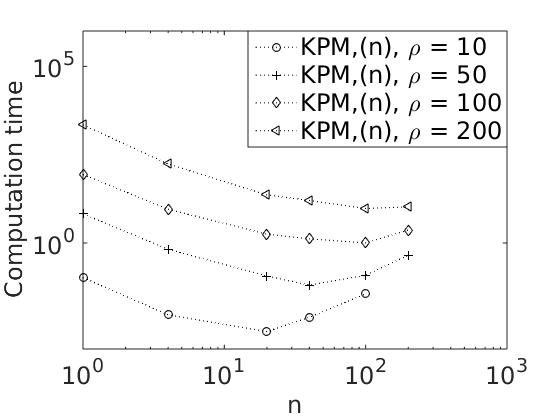
\includegraphics[width=\textwidth]{fig/s9rest1}
                \caption{function \texttt{P1}}
                \label{fig:rest1}
        \end{subfigure}
~
        \begin{subfigure}[b]{0.45\textwidth}
                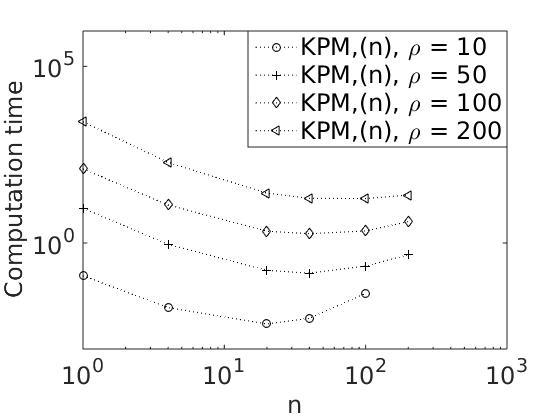
\includegraphics[width=\textwidth]{fig/s10rest2}
                \caption{function \texttt{P2}}
                \label{fig:rest2}
        \end{subfigure}
        \caption{Computation time plotted against restart variable $n$.}\label{fig:rest}
\end{figure}
As can be see from figure \ref{fig:rest}, the optimal restart variable changes as a function of $\rho$ so that larger $\rho$ needs larger $n$ to preform optimally, $n = \rho$ seams to give the smallest computation time for the cases tested. One point is missing from KPM$(n)$, $\rho = 10$, this is because the last point plotted is the same as KPM.  
%%%%%%%%%%%%%%%%%%%%%%%%%%%%%%%%%%%%%%%%%%%%%%%%%%%%%%%%%%%%%%%%%%%%%%%%%%%%%%%%%%%%%%%%%%%%%%%%%%%%%%%%%%%%%%%%%%%%%%
\section{Comparing $\gamma$ and $n$} \label{sec:rrest}
%%%%%%%%%%%%%%%%%%%%%%%%%%%%%%%%%%%%%%%%%%%%%%%%%%%%%%%%%%%%%%%%%%%%%%%%%%%%%%%%%%%%%%%%%%%%%%%%%%%%%%%%%%%%%%%%%%%%%%
\begin{figure}[H]
        \centering
        \begin{subfigure}[b]{0.45\textwidth}
                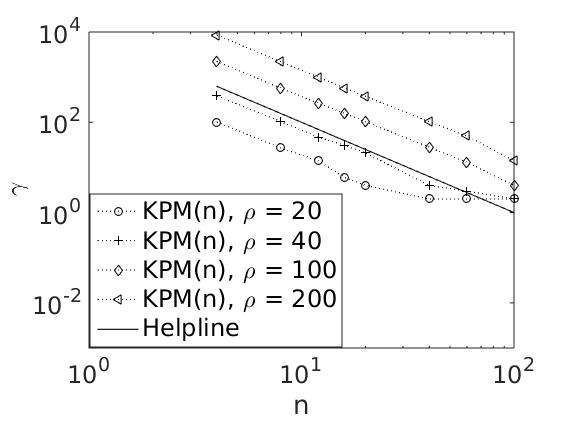
\includegraphics[width=\textwidth]{fig/s3antvsm1}
                \caption{function \texttt{P1}}
                \label{fig:ant1}
        \end{subfigure}%
~
        \begin{subfigure}[b]{0.45\textwidth}
                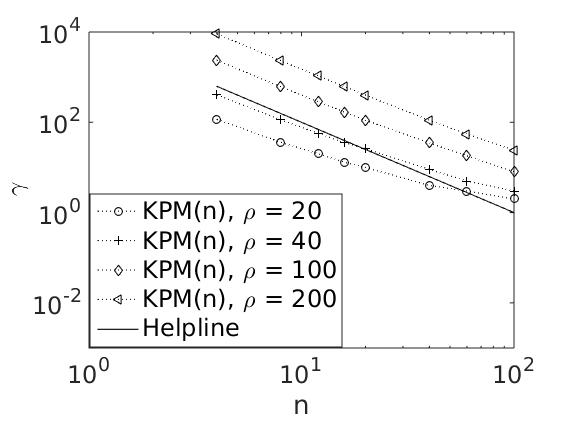
\includegraphics[width=\textwidth]{fig/s4antvsm2}
                \caption{function \texttt{P2}}
                \label{fig:ant2}
        \end{subfigure}
        \caption{The number of restarts, $\gamma$ needed for KPM$(n)$ to converge as a function of the restart variable $n$. The helpline follows $1/n^2$.}\label{fig:ant}
\end{figure}

The helpline from figure \ref{fig:ant} shows that the number of restarts is proportional to $1/n^2$ for all tested cases, if we put this together with the assumption from section \ref{sec:cc} we get that $\gamma \propto  m^2/n^2$. Using table \ref{tab:cc} we get that KPM$(\rho)$ has a complexity of $\mathcal{O}(km^2 + m^3)$ for separable $p$, and $\mathcal{O}(km^3 + m^4)$ for non-separable $p$, which is the same as for KPM.\\

We also see that the number of restarts decrease quickest when $n < \rho $, and slower when $n > \rho$. This is the gain we observed in section \ref{sec:restvar}. On each side of $n = \rho$ we can perform better, either by performing fewer restarts with larger matrices, or more restarts with smaller matrices. \\
%%%%%%%%%%%%%%%%%%%%%%%%%%%%%%%%%%%%%%%%%%%%%%%%%%%%%%%%%%%%%%%%%%%%%%%%%%%%%%%%%%%%%%%%%%%%%%%%%%%%%%%%%%%%%%%%%%%%%%
\section{Computation time with different $\rho$} \label{sec:stimem}
%%%%%%%%%%%%%%%%%%%%%%%%%%%%%%%%%%%%%%%%%%%%%%%%%%%%%%%%%%%%%%%%%%%%%%%%%%%%%%%%%%%%%%%%%%%%%%%%%%%%%%%%%%%%%%%%%%%%%%
\begin{figure}[H]
        \centering
        \begin{subfigure}[b]{0.45\textwidth}
                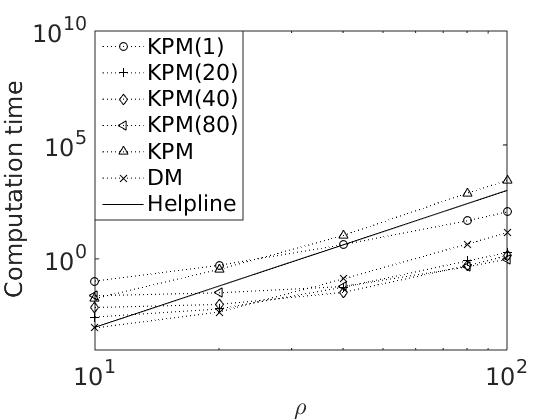
\includegraphics[width=\textwidth]{fig/n5timevsm1}
                \caption{function \texttt{P1}}
                \label{fig:timem1}
        \end{subfigure}%
        ~
        \begin{subfigure}[b]{0.45\textwidth}
                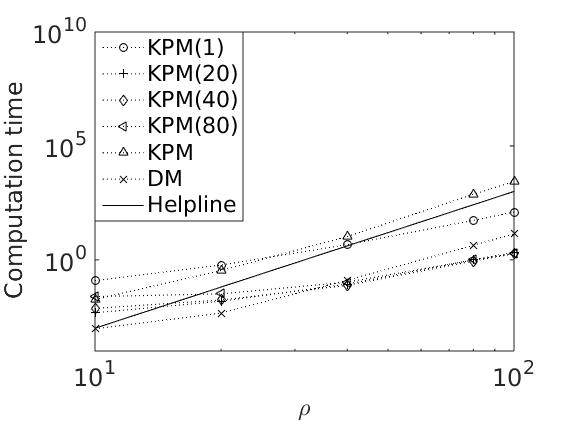
\includegraphics[width=\textwidth]{fig/n6timevsm2}
                \caption{function \texttt{P2}}
                \label{fig:timem2}
        \end{subfigure}
        \caption{A plot of computation time as a function of $\rho$. The helpline increases with $\rho^6 = m^3$.}\label{fig:timem}
\end{figure}
As we can see from figure \ref{fig:timem}, the computation time for KPM increases as expected, while DM and KPM$(n)$ increases slower, perhaps due to MATLAB's efficient inversion algorithm or less memory demand. 
Even more interesting is it that KPM$(n)$ is both asymptotically better, and faster than DM for large $\rho$. Clearly KPM$(n)$ is better in some cases.
%%%%%%%%%%%%%%%%%%%%%%%%%%%%%%%%%%%%%%%%%%%%%%%%%%%%%%%%%%%%%%%%%%%%%%%%%%%%%%%%%%%%%%%%%%%%%%%%%%%%%%%%%%%%%%%%%%%%%%
\section{Computation time with different $k$} \label{sec:stimek}
%%%%%%%%%%%%%%%%%%%%%%%%%%%%%%%%%%%%%%%%%%%%%%%%%%%%%%%%%%%%%%%%%%%%%%%%%%%%%%%%%%%%%%%%%%%%%%%%%%%%%%%%%%%%%%%%%%%%%%
\begin{figure}[H]
        \centering
        \begin{subfigure}[b]{0.45\textwidth}
                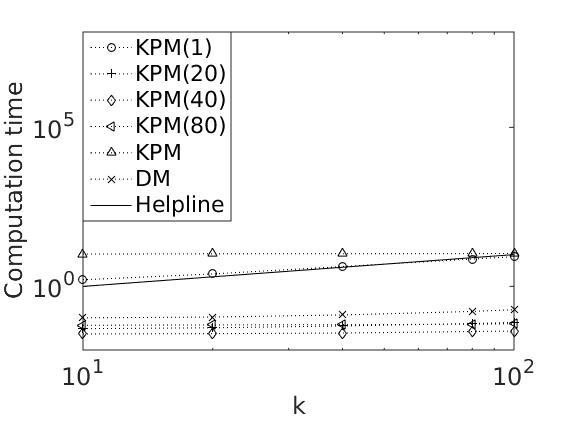
\includegraphics[width=\textwidth]{fig/n7timevsk1}
                \caption{function \texttt{P1}}
                \label{fig:timek1}
        \end{subfigure}%
~
        \begin{subfigure}[b]{0.45\textwidth}
                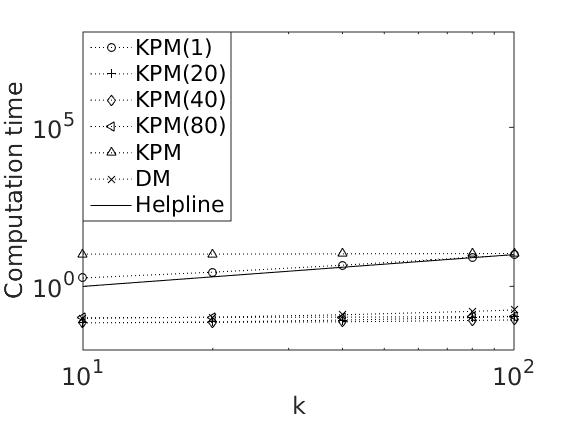
\includegraphics[width=\textwidth]{fig/n8timevsk2}
                \caption{function \texttt{P2}}
                \label{fig:timek2}
        \end{subfigure}
        \caption{A plot of computation time as a function of $k$. The helpline increases with $k$.}\label{fig:timek}
\end{figure}
As we can see from figure \ref{fig:timek}, the computation time for almost all tested methods are constant. The reason is that the time needed for initializing is much greater than the time it takes to integrate. 
The exception is KPM$(1)$, which increases close to linear because relatively more work is done while integrating, due to several restarts. 
We also see that KPM$(n)$ is faster than DM for some $n$, but not asymptotically.

With larger $n$ I expect that all method would follow the helpline.
%%%%%%%%%%%%%%%%%%%%%%%%%%%%%%%%%%%%%%%%%%%%%%%%%%%%%%%%%%%%%%%%%%%%%%%%%%%%%%%%%%%%%%%%%%%%%%%%%%%%%%%%%%%%%%%%%%%%%%
\section{Comparing $\delta$, $\gamma$ and $\epsilon$ } \label{sec:div}
%%%%%%%%%%%%%%%%%%%%%%%%%%%%%%%%%%%%%%%%%%%%%%%%%%%%%%%%%%%%%%%%%%%%%%%%%%%%%%%%%%%%%%%%%%%%%%%%%%%%%%%%%%%%%%%%%%%%%%
Remember that $\delta$ is tolerance, $\gamma$ is the number of restarts, and $\epsilon$ is a measure for the error.
\begin{figure}[H]
        \centering
        \begin{subfigure}[b]{0.45\textwidth}
                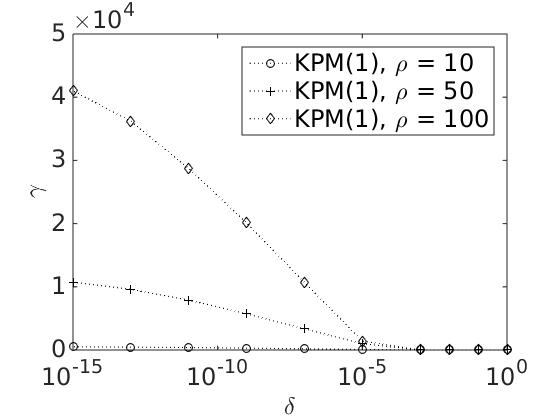
\includegraphics[width=\textwidth]{fig/s13antvstol1m}
                \caption{function \texttt{P1}}
                \label{fig:gammadelta1}
        \end{subfigure}
~
        \begin{subfigure}[b]{0.45\textwidth}
                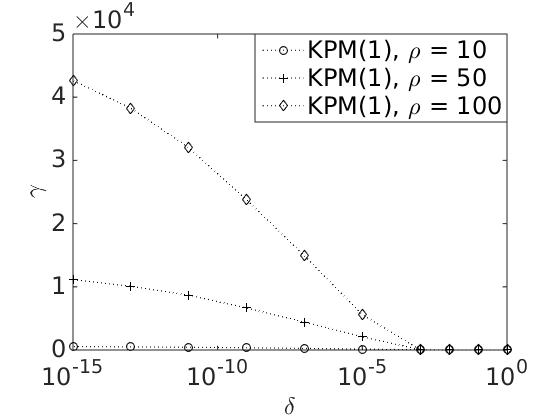
\includegraphics[width=\textwidth]{fig/s14antvstol2m}
                \caption{ function \texttt{P2}}
                \label{fig:gammadelta2}
        \end{subfigure}
        
        \begin{subfigure}[b]{0.45\textwidth}
                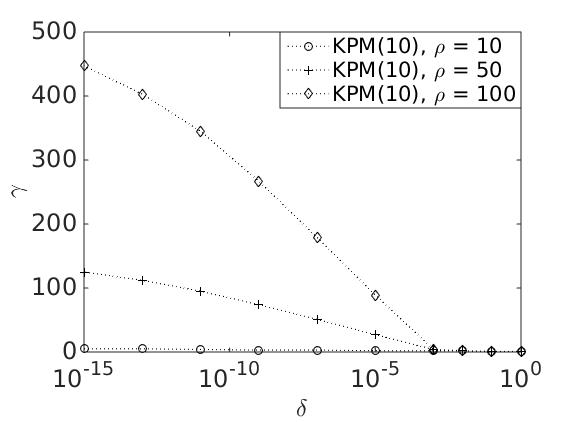
\includegraphics[width=\textwidth]{fig/s13antvstol1m10}
                \caption{function \texttt{P1}}
                \label{fig:gammadelta3}
        \end{subfigure}
~
        \begin{subfigure}[b]{0.45\textwidth}
                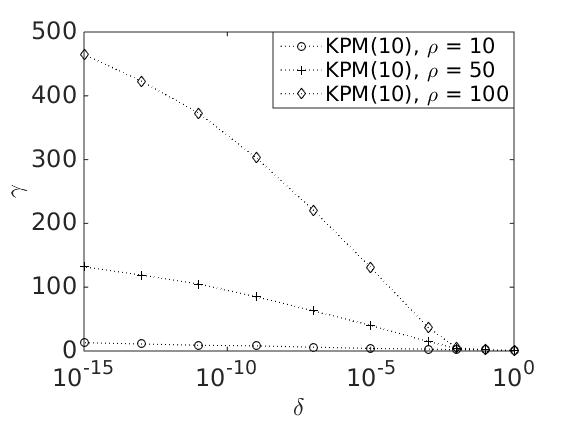
\includegraphics[width=\textwidth]{fig/s14antvstol2m10}
                \caption{ function \texttt{P2}}
                \label{fig:gammadelta4}
        \end{subfigure}
        
        \caption{A plot of $\gamma$ as a function of $\delta$, with several $\rho$ and $n$.} \label{fig:gammadelta}
\end{figure}
We see from figure \ref{fig:gammadelta} that $\gamma$ changes significantly with $\rho$. The figure show a log linear dependence between $\gamma$ and $\delta$, and that $\gamma \propto 1/n^2$. 
The constant part of the graph where $ 10^{-5}<\delta< {10^0} $ shows that KPM$(1)$ and KPM$(10)$ does too few restarts to gain any accuracy when $\delta$ is too large, this is confirmed by figure \ref{fig:epsilondelta}. 

\begin{figure}[H]
        \centering
        \begin{subfigure}[b]{0.45\textwidth}
                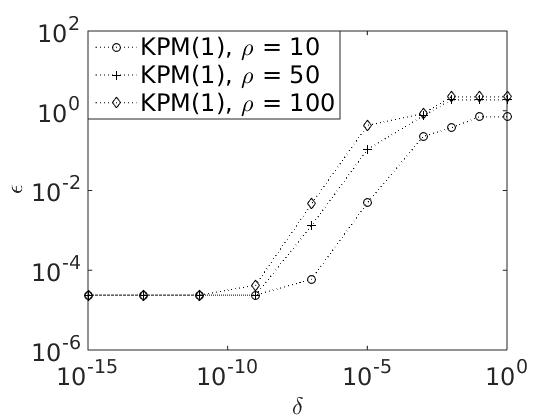
\includegraphics[width=\textwidth]{fig/s15errvstol1m}
                \caption{function \texttt{P1}}
                \label{fig:epsilondelta1}
        \end{subfigure}
~
        \begin{subfigure}[b]{0.45\textwidth}
                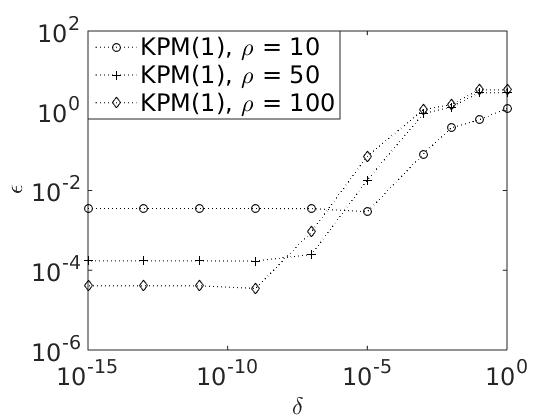
\includegraphics[width=\textwidth]{fig/s16errvstol2m}
                \caption{ function \texttt{P2}}
                \label{fig:epsilondelta2}
        \end{subfigure}
        
        \begin{subfigure}[b]{0.45\textwidth}
                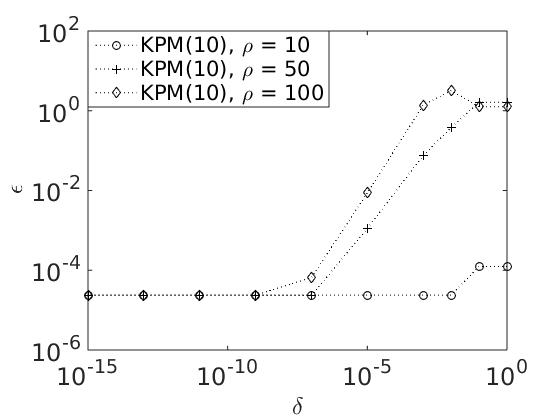
\includegraphics[width=\textwidth]{fig/s15errvstol1m10}
                \caption{function \texttt{P1}}
                \label{fig:epsilondelta3}
        \end{subfigure}
~
        \begin{subfigure}[b]{0.45\textwidth}
                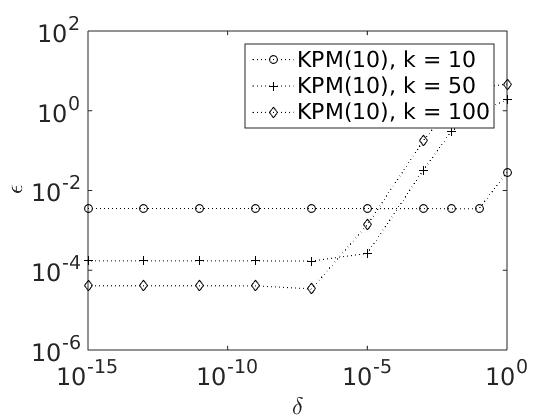
\includegraphics[width=\textwidth]{fig/s16errvstol2m10}
                \caption{ function \texttt{P2}}
                \label{fig:epsilondelta4}
        \end{subfigure}
        
        \caption{A plot of $\epsilon$ as a function of $\delta$, with several $\rho$ and $n$.} \label{fig:epsilondelta}
\end{figure}
Figure \ref{fig:epsilondelta} shows $\epsilon$ as a function of $\delta$. In figure \ref{fig:epsilondelta1} and \ref{fig:epsilondelta3} all graphs has obtained the threshold precision possible with $k=40$. In
figure \ref{fig:epsilondelta2} and \ref{fig:epsilondelta4} the precision possible with the different $\rho$-s are obtained. It seams that the maximum precision is attained faster with larger $n$, this makes sense because if $n = m$, we should not need to restart in order to get threshold precision. This was also confirmed by figure \ref{fig:gammadelta}, where KPM$(10)$ needed fewer restarts than KPM$(1)$ to converge. 
%There is no reason this was not performed with other than $n = 1$ except for laziness. \\
%!!!!!!!!!!!!!!!!!!!!!!!!!Arg, jeg må lage nye figurer for andre $n$!!!!!!!!!!!!!!!!!!!!!!!!!!!!!!!!!!\\
%!!!!!!!!!!!!!!!!Her kan burde skrive noe om hvor bra KPM$(n)$ uten restart ville vært!!!!!!!!!!!!!!!!\\
%!!!!!!!!!!!!!!!!!!!!!Fjern alle forekomster av ordet "shows" fra avsnittet!!!!!!!!!!!!!!!!!!!!!!!!!!!!\\
%!!!!!!!!!!!!!!!!!!!!!Forklare hva alle variablene er over alt!!!!!!!!!!!!!!!!!!!!!!!!!!\\
%!!!!!!!!!!!!!!!!!!!!!Skrive hvorfor vi ikke har med noe annet enn KPM$(1)$!!!!!!!!!!!!!!!!!!\\
%!!!!!!!!!!!!!!!!!!!!!!!!!!!Går videre så jeg ikke trenger å lage nye figurer med en gang!!!!!!!!!!!!!!!!!!!!!!!!!!\\
%Figure \ref{fig:errant} and \ref{fig:errtolk} shows how $\gamma$ and $\epsilon$ scales with $\delta$. Figure \ref{fig:errtol1} has reached to threshold precision with $k = 40$. Both figures shows a loglinear dependence between $\gamma$ and $\delta$. The figures also shows the importance of choosing an appropriate $\delta$. A lot of time can be saved by choosing $\delta$ larger, but precision is lost if $\delta$ is to large.
\begin{figure}[H]
        \centering
        \begin{subfigure}[b]{0.45\textwidth}
                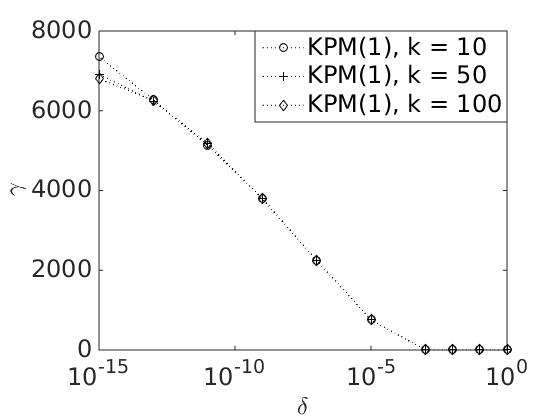
\includegraphics[width=\textwidth]{fig/s20antvstol1k}
                \caption{function \texttt{P1}}
                \label{fig:gammadeltak1}
        \end{subfigure}
~
        \begin{subfigure}[b]{0.45\textwidth}
                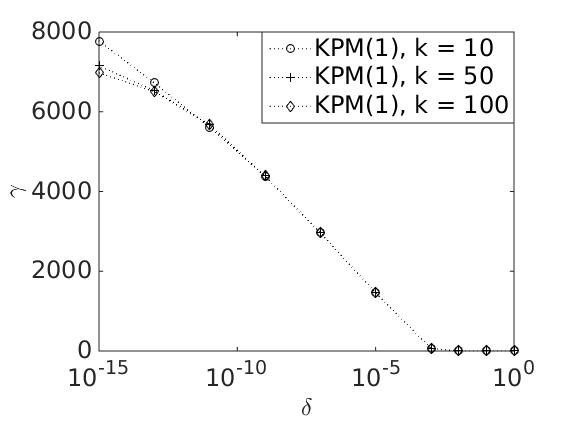
\includegraphics[width=\textwidth]{fig/s21antvstol2k}
                \caption{ function \texttt{P2}}
                \label{fig:gammadeltak2}
        \end{subfigure}
                \begin{subfigure}[b]{0.45\textwidth}
                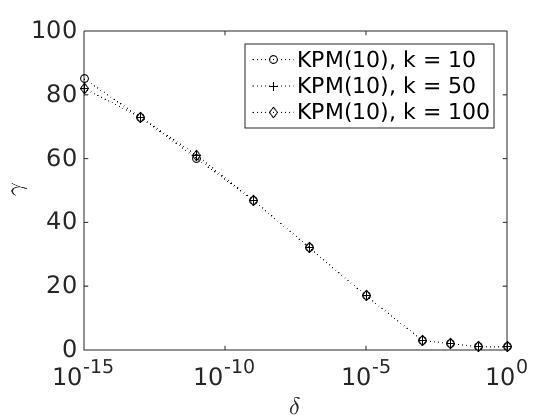
\includegraphics[width=\textwidth]{fig/s20antvstol1k10}
                \caption{function \texttt{P1}}
                \label{fig:gammadeltak3}
        \end{subfigure}
~
        \begin{subfigure}[b]{0.45\textwidth}
                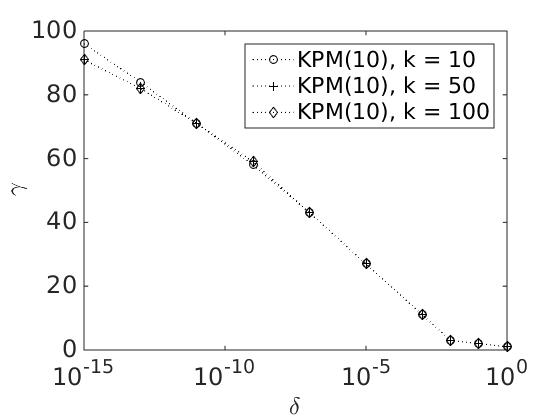
\includegraphics[width=\textwidth]{fig/s21antvstol2k10}
                \caption{ function \texttt{P2}}
                \label{fig:gammadeltak4}
        \end{subfigure}
        \caption{A plot of $\gamma$ as a function of $\delta$, with several $k$ and $n$.} \label{fig:gammadeltak}
\end{figure}
Figure \ref{fig:gammadeltak} shows that $\gamma$ is nearly independent of $k$. The figures also shows the log linear dependence between $\delta$ and $\gamma$. \\



\begin{figure}[H]
        \centering
        \begin{subfigure}[b]{0.45\textwidth}
                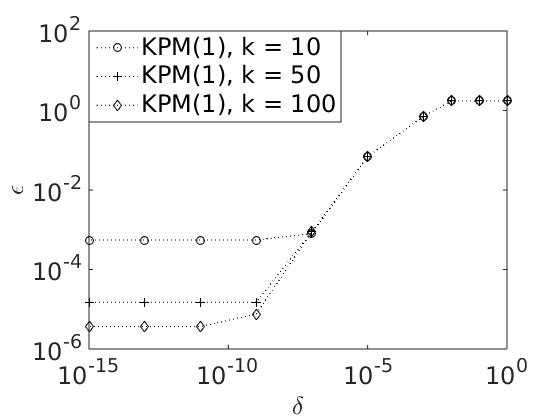
\includegraphics[width=\textwidth]{fig/s22errvstol1k}
                \caption{function \texttt{P1}}
                \label{fig:epsilondelta1k}
        \end{subfigure}
~
        \begin{subfigure}[b]{0.45\textwidth}
                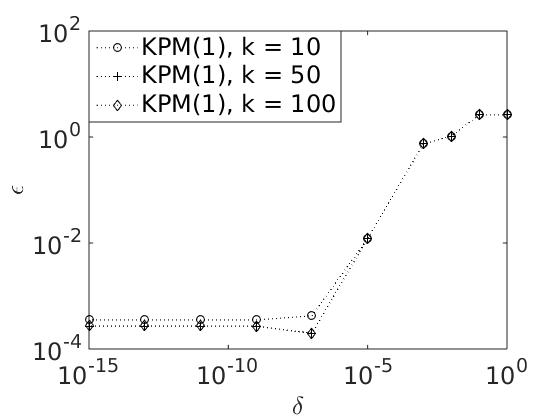
\includegraphics[width=\textwidth]{fig/s23errvstol2k}
                \caption{ function \texttt{P2}}
                \label{fig:epsilondelta2k}
        \end{subfigure}
                \begin{subfigure}[b]{0.45\textwidth}
                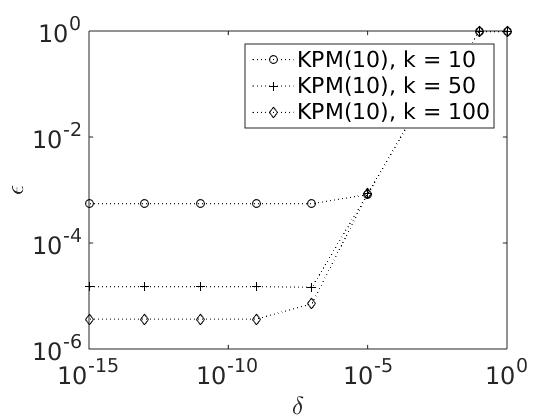
\includegraphics[width=\textwidth]{fig/s22errvstol1k10}
                \caption{function \texttt{P1}}
                \label{fig:epsilondelta3k}
        \end{subfigure}
~
        \begin{subfigure}[b]{0.45\textwidth}
                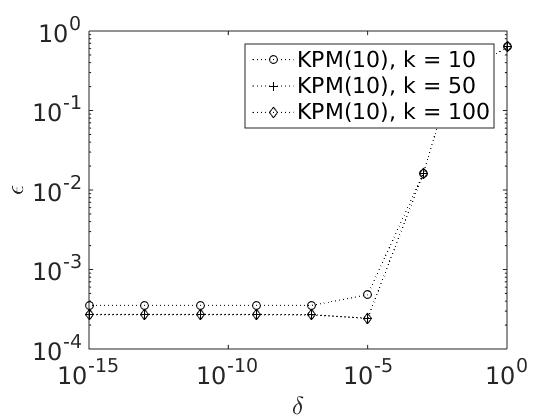
\includegraphics[width=\textwidth]{fig/s23errvstol2k10}
                \caption{ function \texttt{P2}}
                \label{fig:epsilondelta4k}
        \end{subfigure}
        \caption{A plot of $\epsilon$ as a function of $\delta$, with several $k$ and $n$.} \label{fig:epsilondeltak}
\end{figure}
Figure \ref{fig:epsilondeltak} shows much the same as figure \ref{fig:epsilondelta}. Maximum precision for different $k$ is shown in figure \ref{fig:epsilondelta1k} and \ref{fig:epsilondelta3k}.
Threshold precision for $\rho = 40$ is obtained in figure \ref{fig:epsilondelta2k} and \ref{fig:epsilondelta4k}, but not for the graph where $k = 10$, this is the precision possible with $k=10$. Again $\epsilon$ converges faster for KPM$(10)$ than KPM$(1)$. \\

We see that there is no gain in precision with increasing one of either $\rho$ or $k$ or decreasing $\delta$ without changing the others appropriately. \\

%Before the constant part, $\epsilon$ is decided by $\delta$ alone. 
In all cases a lot of time can be saved by choosing $\delta$ appropriate. If $\delta$ is to large we get inaccurate answers, if $\delta$ is to small we perform to many restarts to use the algorithm efficiently. There does not seam to be a simple rule to choose $\delta$, since the results for \texttt{P1} and \texttt{P2} differs. The rule I will use is to start at $\delta=10^{-3}$, with $\rho = k = 10$ and decrease $\delta$ with two order of magnitude each time $k$ and $\rho$ is doubled, the reason for this rule is perhaps easier to understand when looking at figure \ref{fig:conv}.